% !TeX root = ../../tfg.tex
% !TeX encoding = utf8
%
%*******************************************************
% Qué es el aprendizaje automático
%*******************************************************

\section{Concepto de aprendizaje}\label{ch:Aprendizaje}

Las redes neuronales son un tipo de algoritmos de Aprendizaje Automático. Por ello, no sería prudente exponer la historia de las redes neuronales sin dar en primer lugar una nociones básicas del área del saber a la que pertenecen.

El término de Aprendizaje Automático 
\cite{hisour} 
fue acuñado en 1959 por Arthur Samuel 
para hacer referencia a los sistemas informáticos que 
pueden <<aprender>> por sí mismos, es decir, mejorar su 
eficacia y rendimiento de forma autónoma a partir de los datos, 
sin que en esas mejoras intervenga un programador.

\begin{marginfigure}
    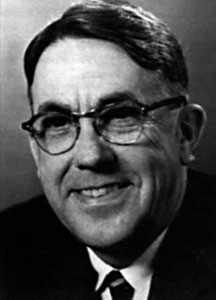
\includegraphics[width=\marginparwidth]{introduccion_redes_neuronales/aprendizaje_introduccion/arthur_samuel.jpg}
    \caption{Arthur L. Samuel (1901-1990) }
    \cite{samuel-wikipedia}
    \small
     se graduó en Ingeniería Electrónica en el MIT. 
     Trabajó en los laboratorios Bell, la Universidad de Illinois,
      en IBM y en la Universidad de Stanford (1966). 
      Fue un pionero de los videojuegos y la inteligencia artificial. 
      Popularizó el término <<Machine Learning>> en 1959. 
      Implementó una IA para jugar a las damas, el primer caso  
      de éxito en aprendizaje automático. Contribuyó notablemente 
      en el desarrollo de TeX.
\end{marginfigure}

Fue en 1997 cuando Tom Mitchell propuso una definición 
más formal de aprendizaje 
\cite{tom-michell-machine-learning}, 
aproximada a la dada en el libro \textit{Learning from data}
\cite{learning-from-data-1-2}, que expondremos en seguida.

El aprendizaje es un proceso por el cual se estima una dependencia desconocida 
(input-output) o la estructura de un sistema a partir de un número finito de 
observaciones.  El aprendizaje se compone de tres elementos principales: 

\begin{itemize}
    \item Un generado o función de distribución de la cual se extraen 
    vectores aleatorios 
    $x \in \mathbb R^ n$ 
    que dependen de una función de densidad desconocida \footnote{De hecho, encontrar esta función resolvería el problema de aprendizaje}.
    
    \item Un sistema que produce un vector de salida $y$ por cada entrada del vector $x$ a partir del valor fijo $p(y|x)$, que es desconocido también. 
    
    \item Una \textit{learning machine}, que en el caso más general no es  más que un conjunto de funciones abstractas cuyos elementos son de la forma $f(x,w), w\in \omega$.
\end{itemize}

\begin{marginfigure}
    
\includegraphics[width=\marginparwidth]{introduccion_redes_neuronales/aprendizaje_introduccion/tom_mitchell.jpg}
   \caption{Tom M. Mitchell}
   \small
    Tom M. Mitchell
     \cite{mitchell-wikipedia} 
    (1951) estudió Ingeniería Electrónica en el MIT, 
    se doctoró en la Universidad de Stanford y ejerce en la Universidad de Carnegie Mellon. Es conocido por su libro 
    de texto Machine Learning. Ha recibido numerosas condecoraciones y 
   participa en asociaciones que promueven la ciencia y la ingeniería.
\end{marginfigure}



Así pues, el objetivo del aprendizaje automático es encontrar una función que se aproxime a la función de densidad desconocida.

Por lo general la teoría se fundamenta en minimizar el error de estimadores, como el error cuadrático medio, ya que este se trata de un UMVUE  (estimador insesgado de mínima varianza). 

$$ECM = \frac{1}{n} \sum_{i=0} ^n (f(x_i) - y_i)^2,$$

donde $f(x_i)$ representa la predicción y $y_i$ la etiqueta de entrenamiento de $x_i$, es decir, su valor real. 

